% PREVIEW: All 4 Setup Charts + All 4 Problem Framings
% For user to choose which approach to use
% November 9, 2025

\documentclass[8pt,aspectratio=169]{beamer}
\usetheme{Madrid}
\usepackage{graphicx}

\definecolor{mlpurple}{RGB}{51,51,178}
\definecolor{mllavender}{RGB}{173,173,224}
\setbeamercolor{structure}{fg=mlpurple}

\title{PREVIEW: Choose Your Approach}
\subtitle{4 Setup Charts + 4 Problem Framings}
\date{November 9, 2025}

\begin{document}

\begin{frame}
\titlepage
\end{frame}

% ============================================
% SECTION 1: 4 SETUP CHART OPTIONS
% ============================================

\begin{frame}{SECTION 1: Setup Charts (Choose 1 of 4)}
\begin{center}
\Large
4 ways to show ``The cat \_\_'' probability problem

\vspace{5mm}
Next 4 slides show all options
\end{center}
\end{frame}

\begin{frame}{Setup Option A: Bar Chart}
\begin{center}
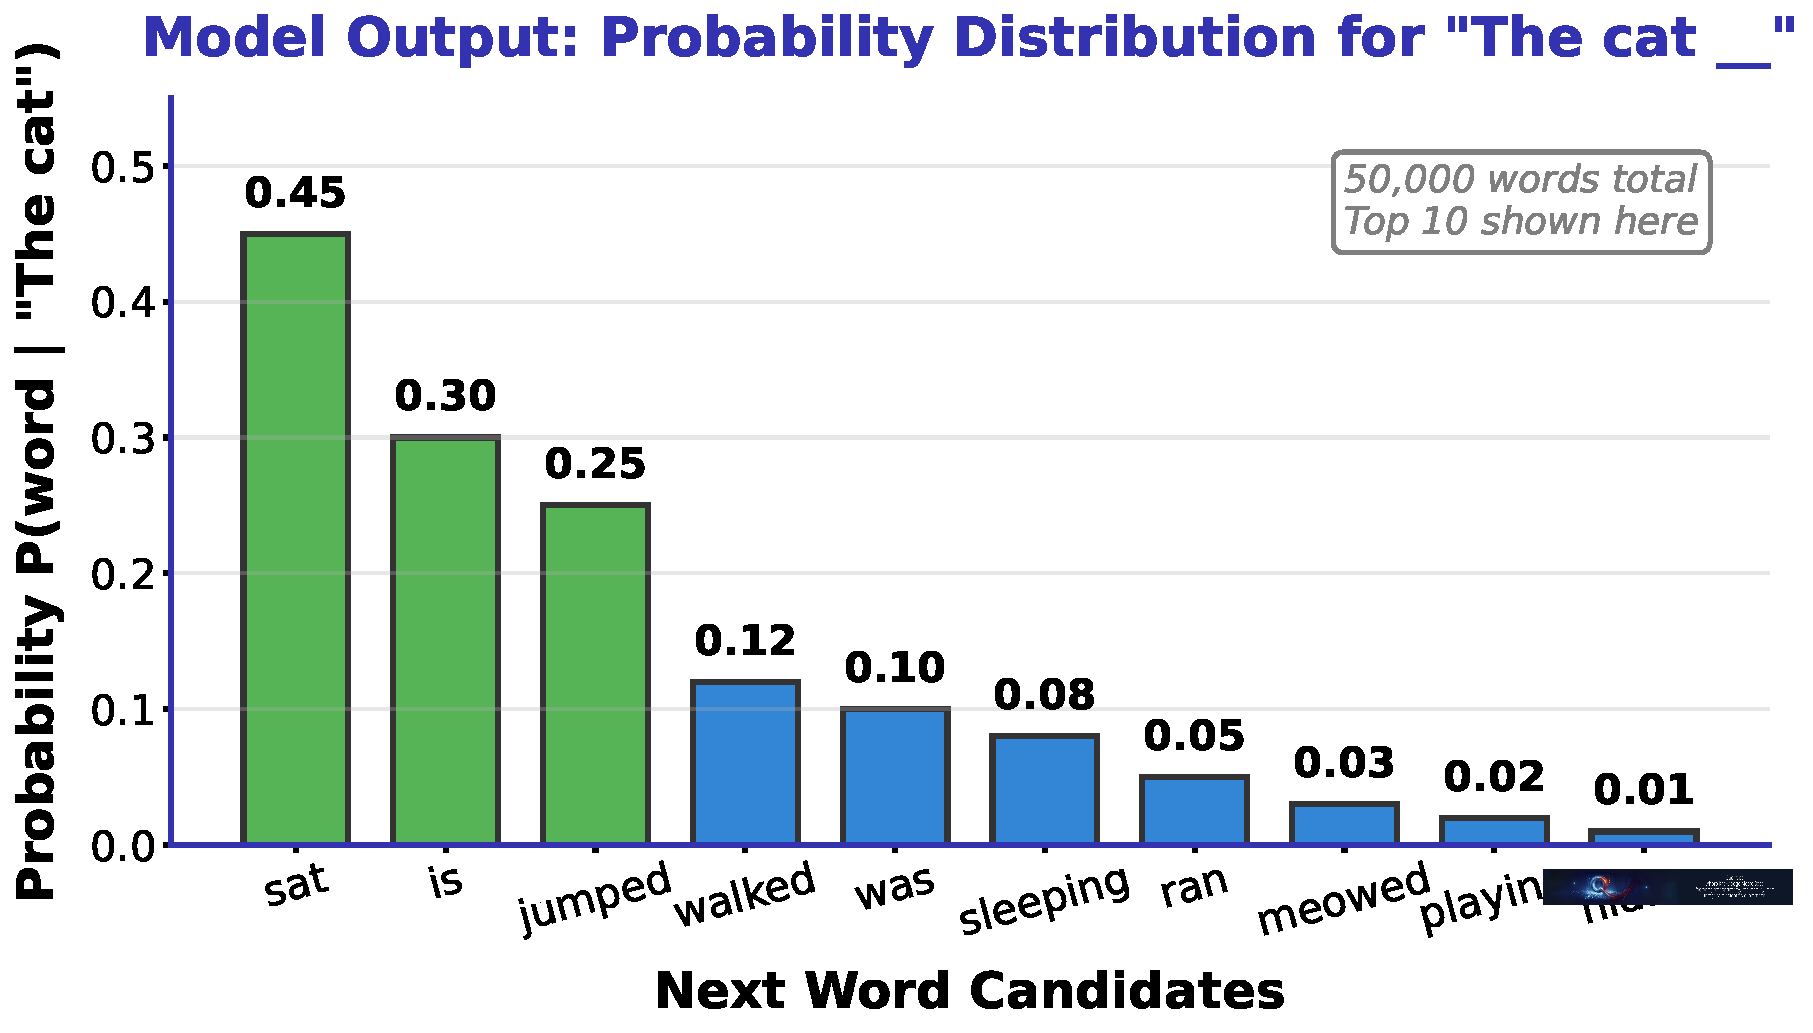
\includegraphics[width=0.75\textwidth]{../figures/setup_A_bar_chart.pdf}
\end{center}
\begin{center}
\textbf{Pros}: Visual, shows distribution clearly

\textbf{Cons}: Takes more space
\end{center}
\end{frame}

\begin{frame}{Setup Option B: List Format}
\begin{center}
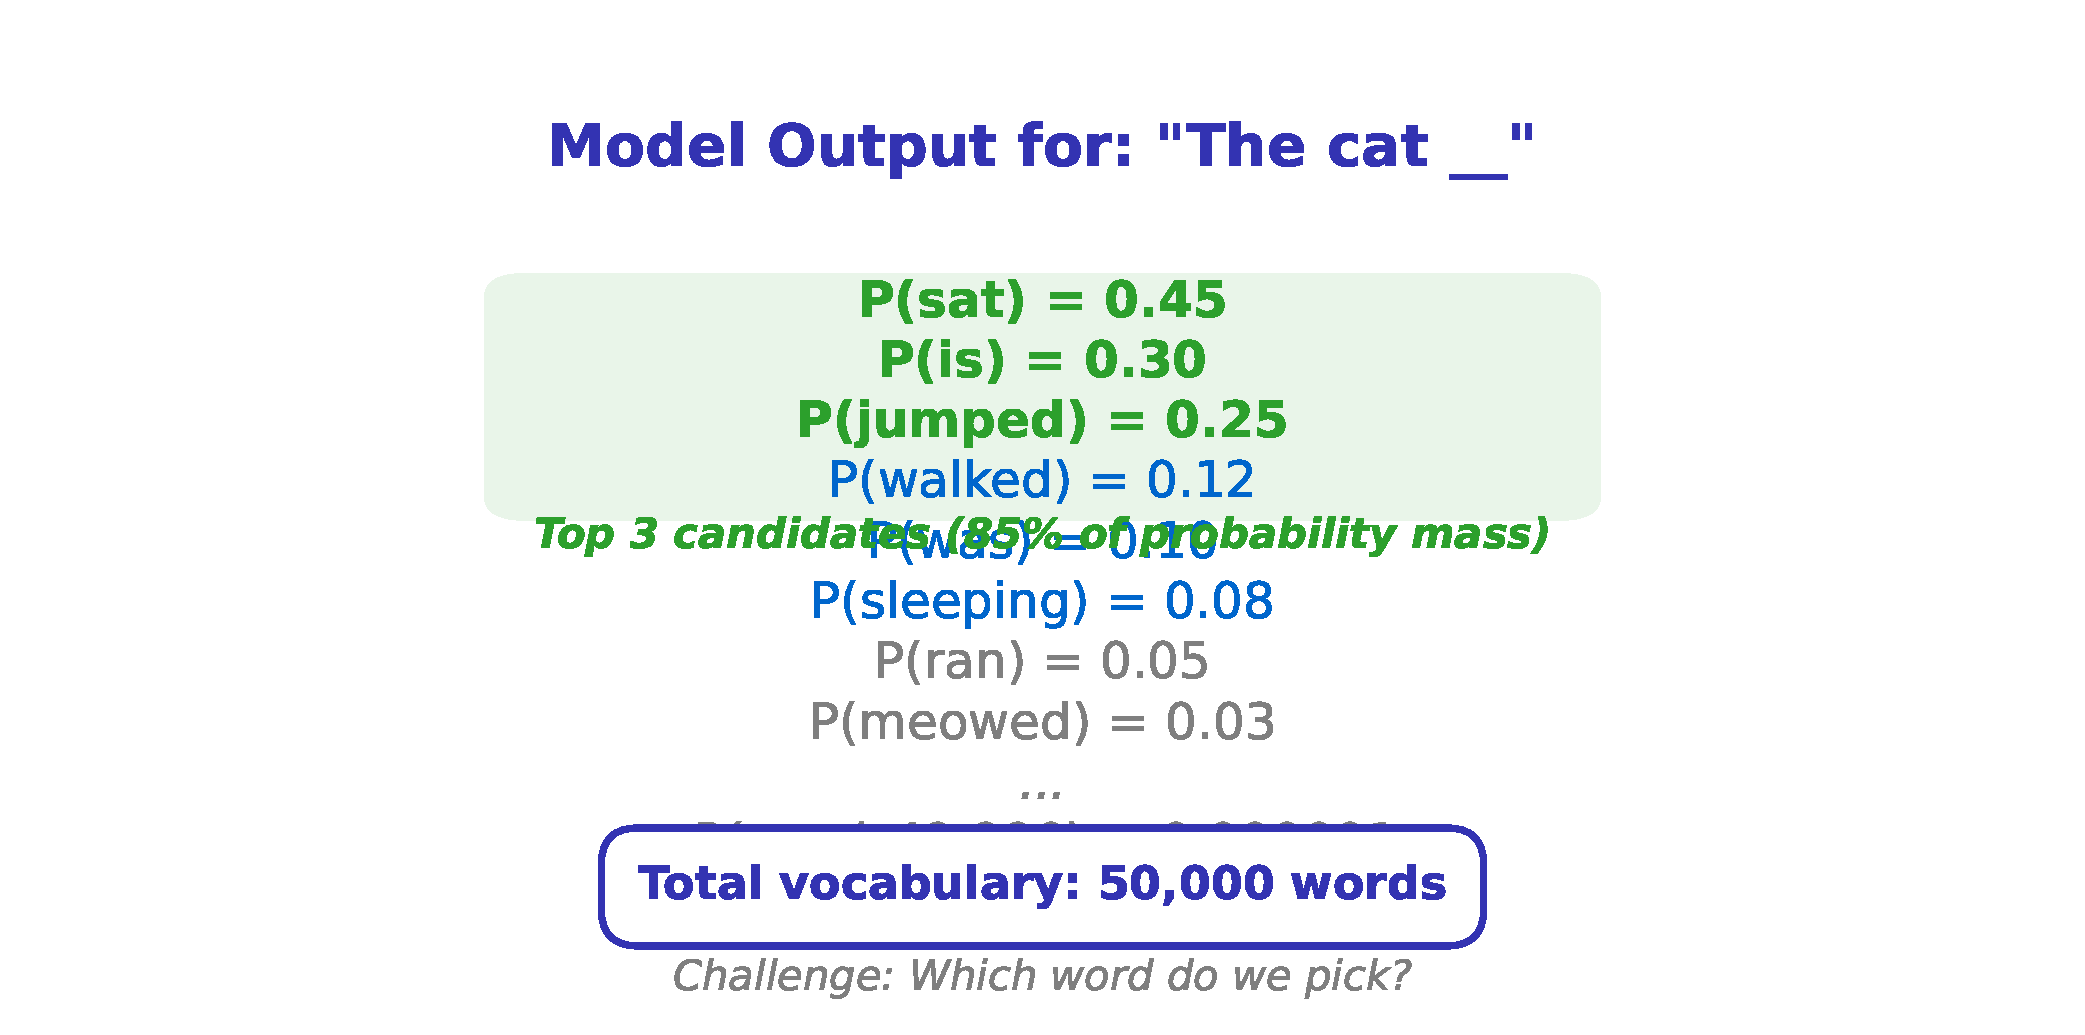
\includegraphics[width=0.75\textwidth]{../figures/setup_B_list.pdf}
\end{center}
\begin{center}
\textbf{Pros}: Clean, simple, text-focused

\textbf{Cons}: Less visual
\end{center}
\end{frame}

\begin{frame}{Setup Option C: Distribution Curve}
\begin{center}
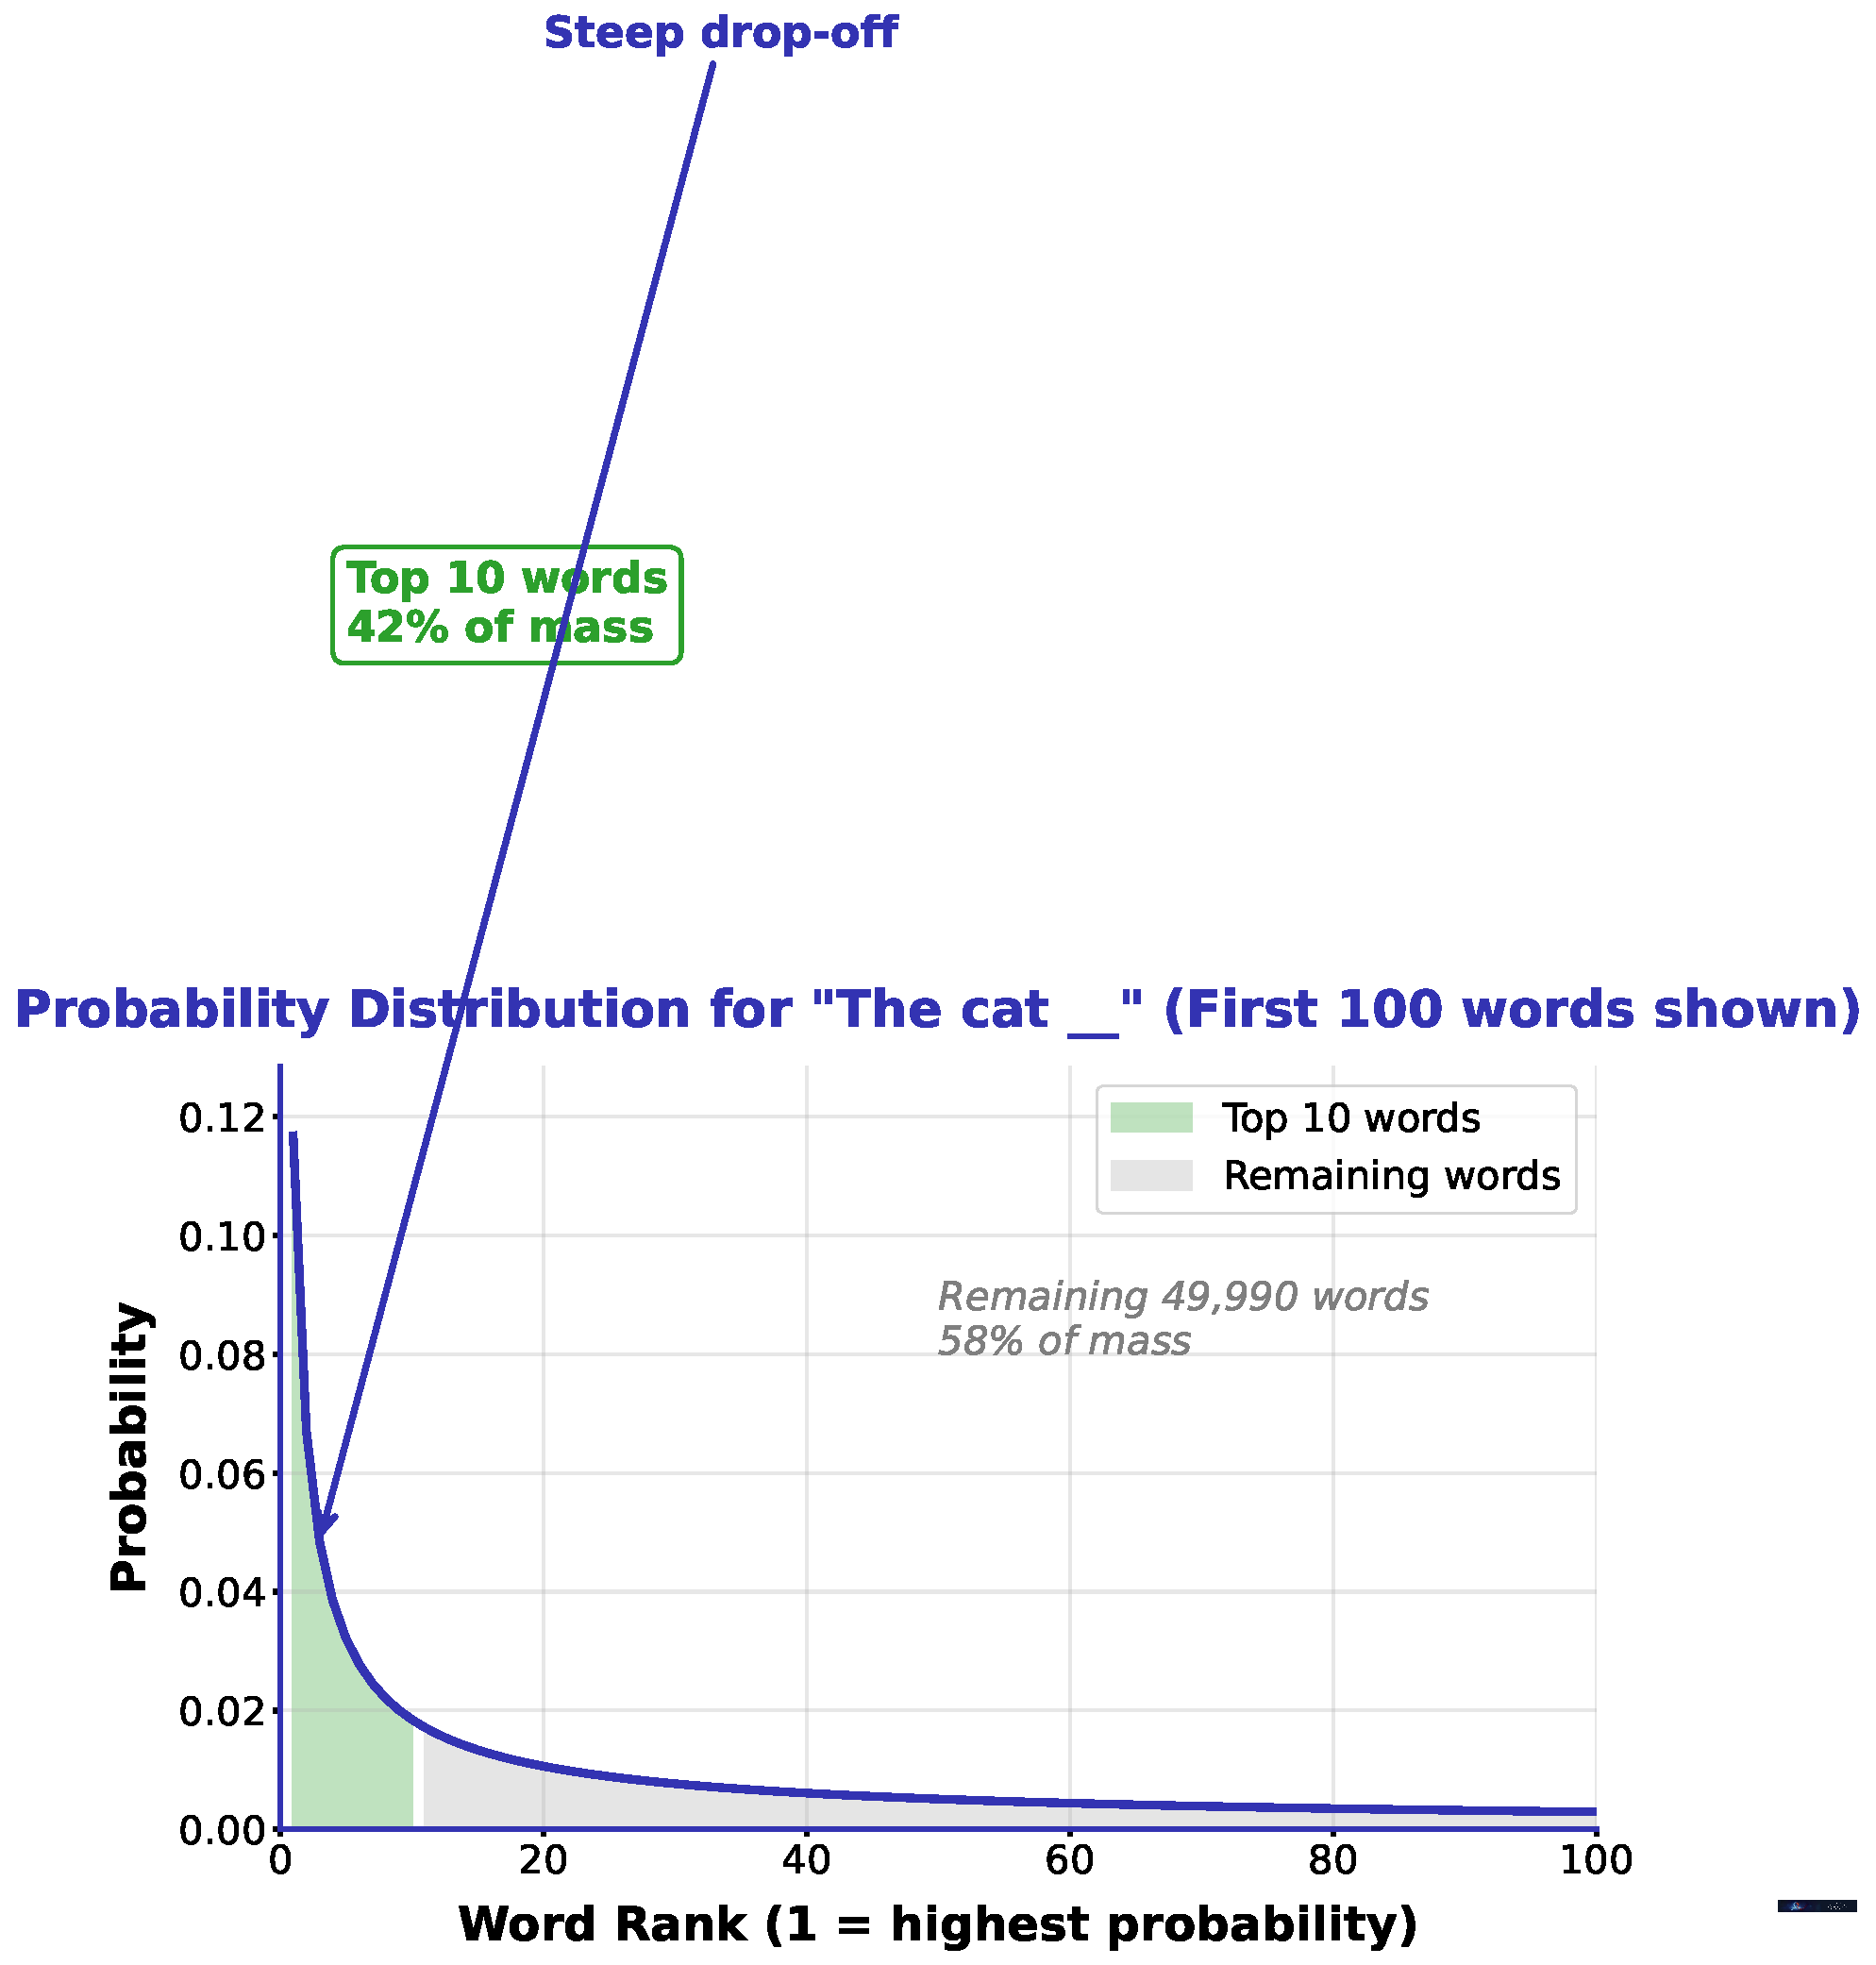
\includegraphics[width=0.75\textwidth]{../figures/setup_C_curve.pdf}
\end{center}
\begin{center}
\textbf{Pros}: Shows power law, emphasizes drop-off

\textbf{Cons}: More abstract
\end{center}
\end{frame}

\begin{frame}{Setup Option D: Node Diagram}
\begin{center}
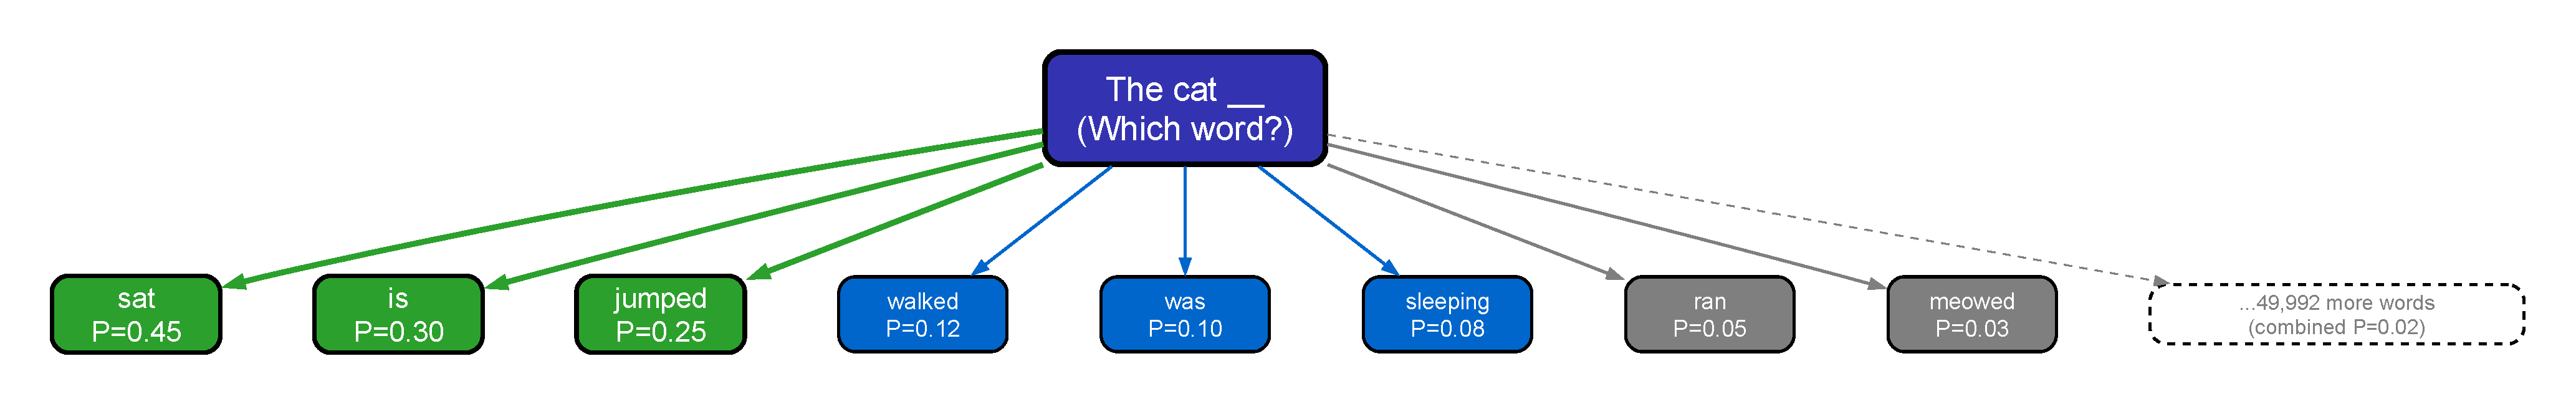
\includegraphics[width=0.65\textwidth]{../figures/setup_D_nodes.pdf}
\end{center}
\begin{center}
\textbf{Pros}: Decision tree style, shows choices

\textbf{Cons}: More complex layout
\end{center}
\end{frame}

% ============================================
% SECTION 2: FRAMING 1 - FAILURE MODES
% ============================================

\begin{frame}{SECTION 2A: Framing 1 - Failure Modes}
\begin{center}
\Large
Frame as: ``What goes wrong and how to fix it''

\vspace{5mm}
6 failure modes → 6 solutions

\vspace{5mm}
Next 6 slides show this framing
\end{center}
\end{frame}

\begin{frame}{Framing 1, Problem 1: Repetitive Loops}
\begin{columns}
\column{0.48\textwidth}
\textbf{Problem}:

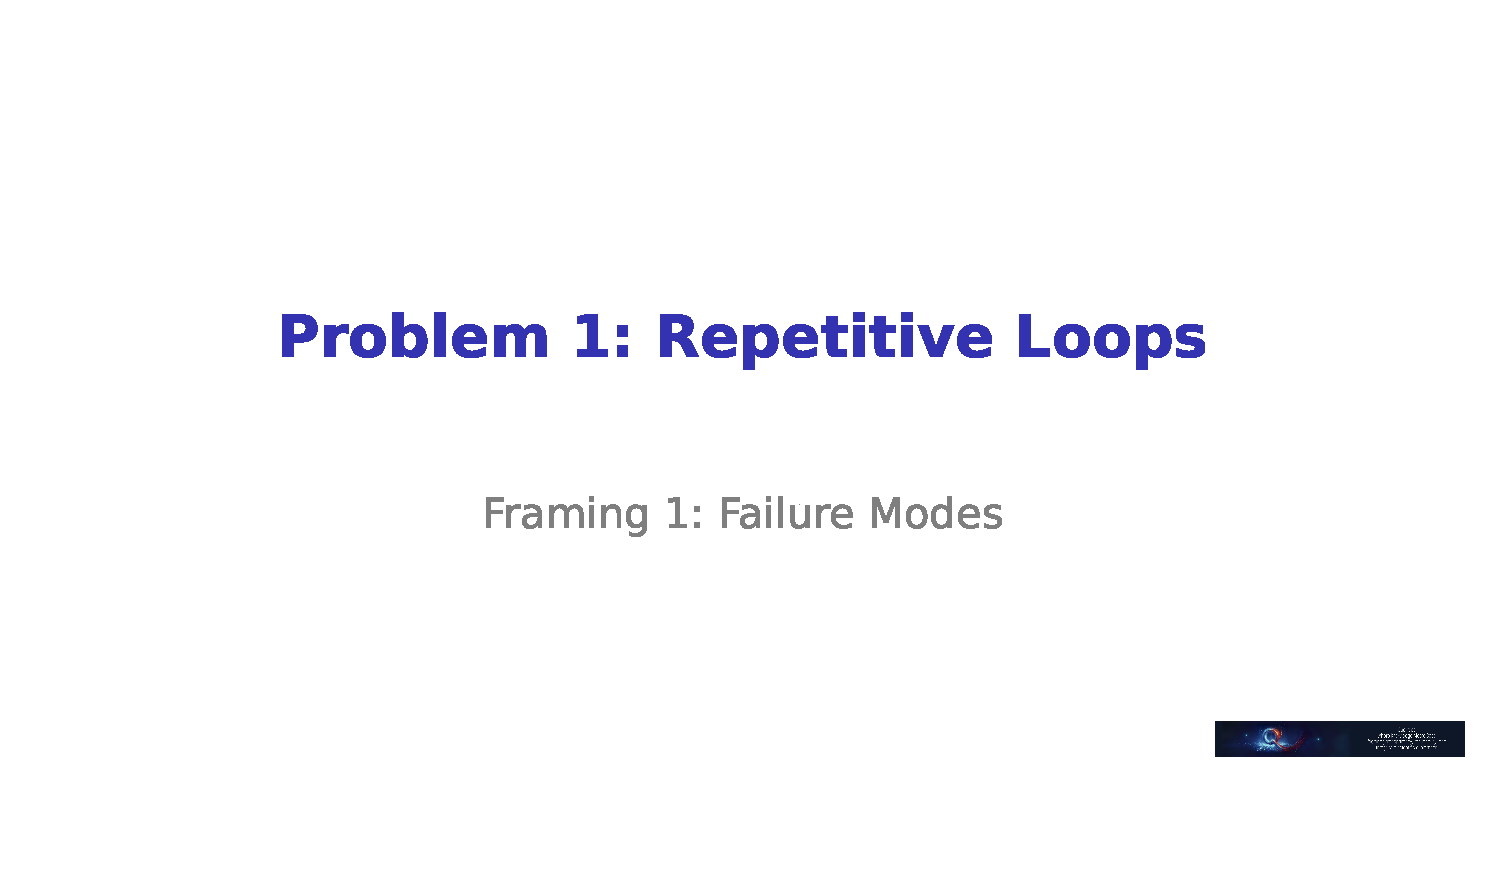
\includegraphics[width=0.95\textwidth]{../figures/framing1_problem1_repetition_loops.pdf}

``The city is a major city in a city...''

Greedy gets stuck in loops

\column{0.48\textwidth}
\textbf{Solution}: \textcolor{mlpurple}{\textbf{BEAM SEARCH}}

Explores multiple paths

Finds better sequences

Width = 3-5 typical

\vspace{3mm}
\colorbox{green!20}{Avoids local optima}
\end{columns}
\end{frame}

\begin{frame}{Framing 1, Problem 2: No Diversity}
\begin{columns}
\column{0.48\textwidth}
\textbf{Problem}:


\includegraphics[width=0.95\textwidth]{../figures/framing1_problem2_no_diversity.pdf}

Always same output

Deterministic = boring

\column{0.48\textwidth}
\textbf{Solution}: \textcolor{mlpurple}{\textbf{TEMPERATURE}}

Adds randomness

T $<$ 1: focused

T $>$ 1: creative

\vspace{3mm}
\colorbox{green!20}{Continuous control over creativity}
\end{columns}
\end{frame}

\begin{frame}{Framing 1, Problem 3: Tail Sampling}
\begin{columns}
\column{0.48\textwidth}
\textbf{Problem}:

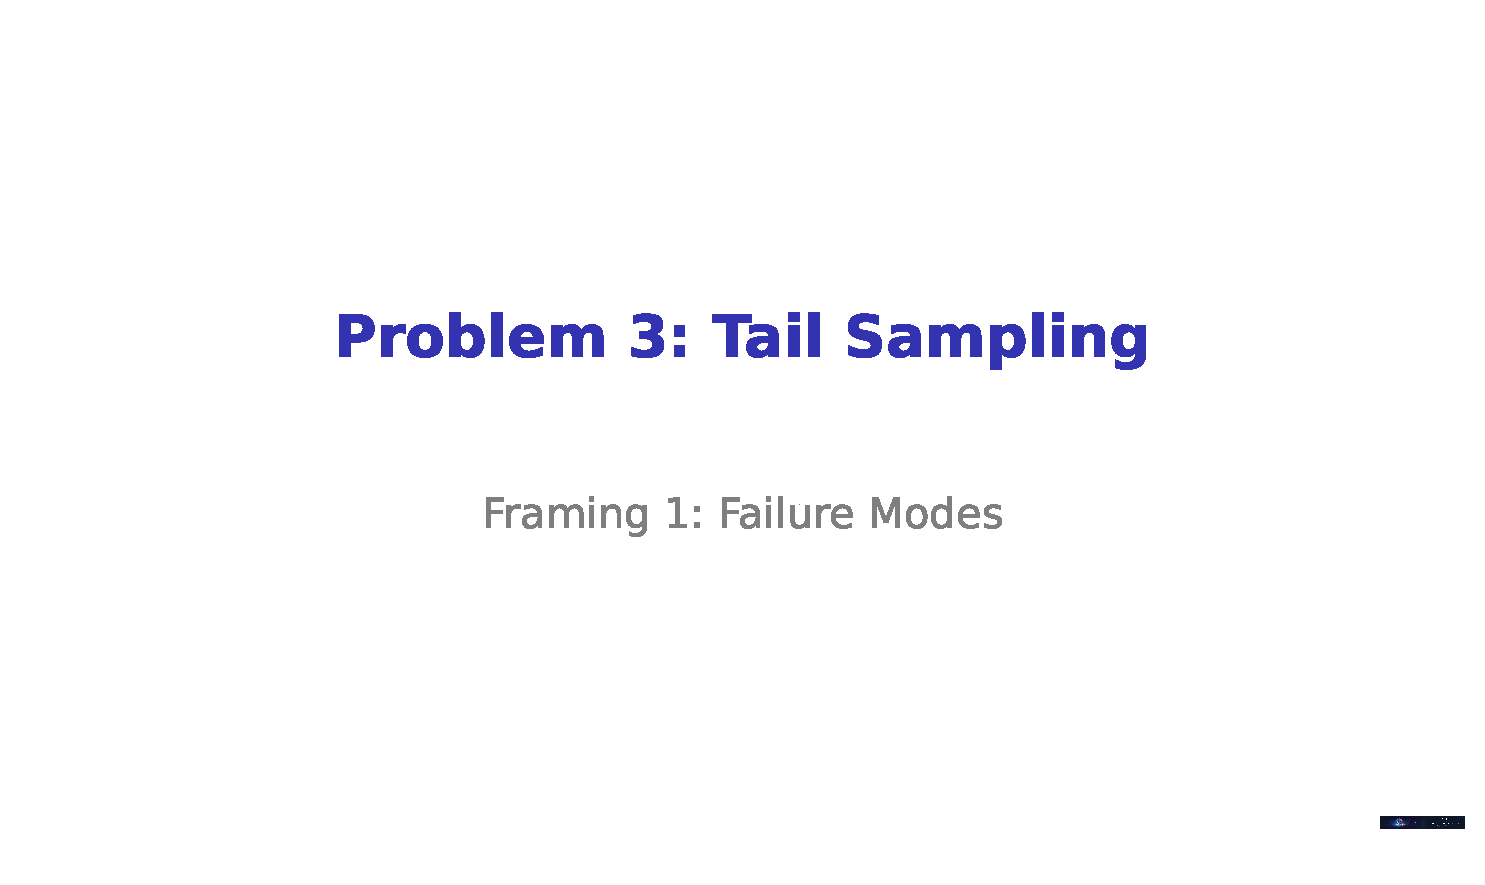
\includegraphics[width=0.95\textwidth]{../figures/framing1_problem3_tail_sampling.pdf}

Random samples unlikely words

``purple flying mathematics''

\column{0.48\textwidth}
\textbf{Solution}: \textcolor{mlpurple}{\textbf{TOP-K}}

Filter bottom 99\%

Sample from top-k only

k = 40-50 typical

\vspace{3mm}
\colorbox{green!20}{Prevents nonsense sampling}
\end{columns}
\end{frame}

\begin{frame}{Framing 1, Problem 4: Fixed Cutoff}
\begin{columns}
\column{0.48\textwidth}
\textbf{Problem}:

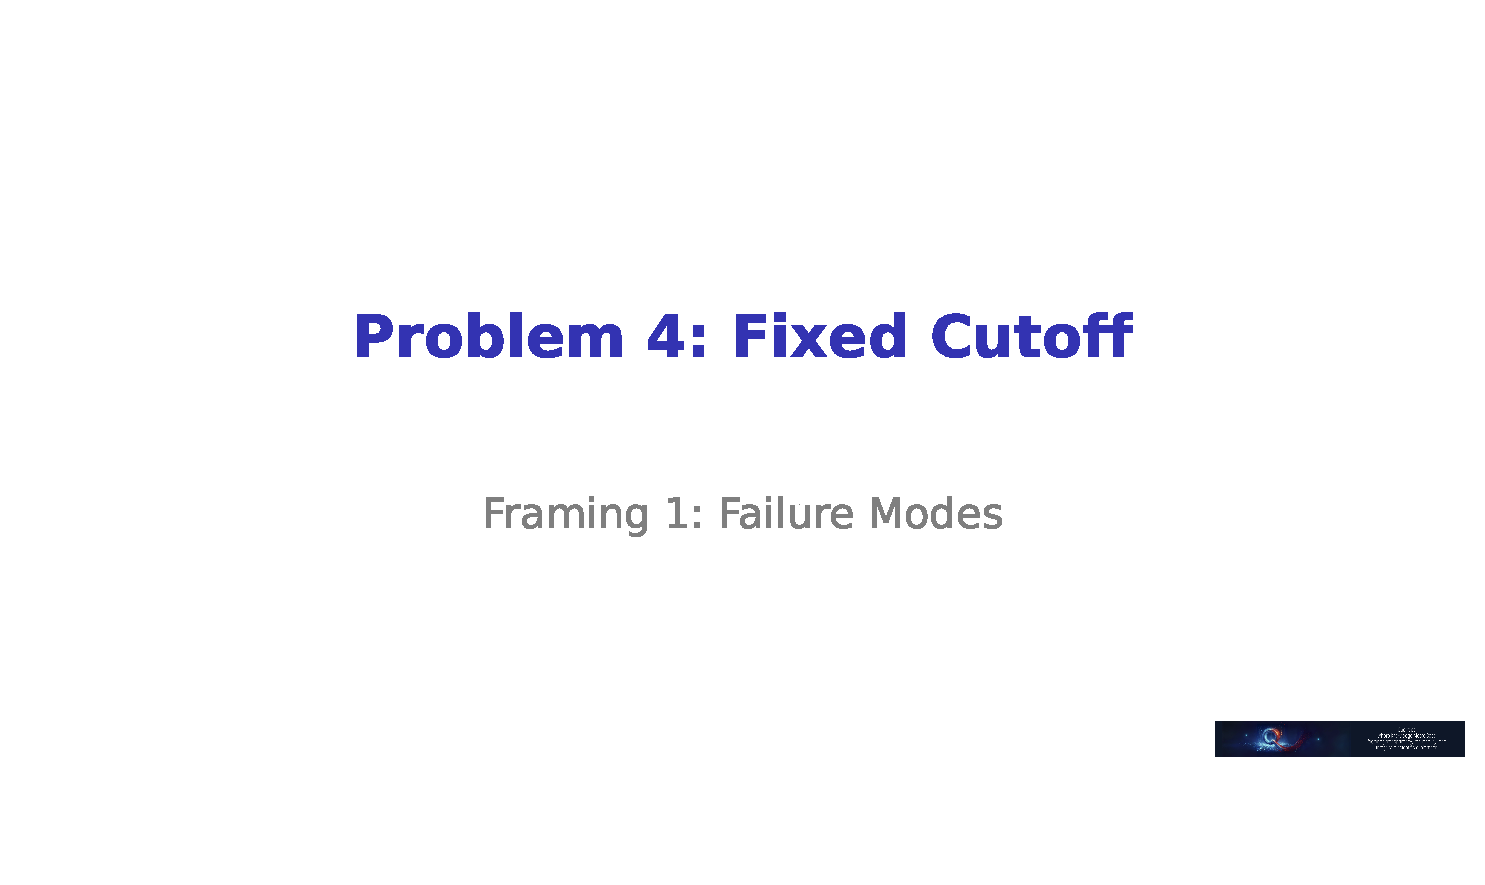
\includegraphics[width=0.95\textwidth]{../figures/framing1_problem4_fixed_cutoff.pdf}

Top-k inflexible

Same k for peaked and flat

\column{0.48\textwidth}
\textbf{Solution}: \textcolor{mlpurple}{\textbf{NUCLEUS (TOP-P)}}

Dynamic cutoff

Adapts to distribution

p = 0.9 typical

\vspace{3mm}
\colorbox{green!20}{Smart filtering}
\end{columns}
\end{frame}

\begin{frame}{Framing 1, Problem 5: Long Degeneration}
\begin{columns}
\column{0.48\textwidth}
\textbf{Problem}:

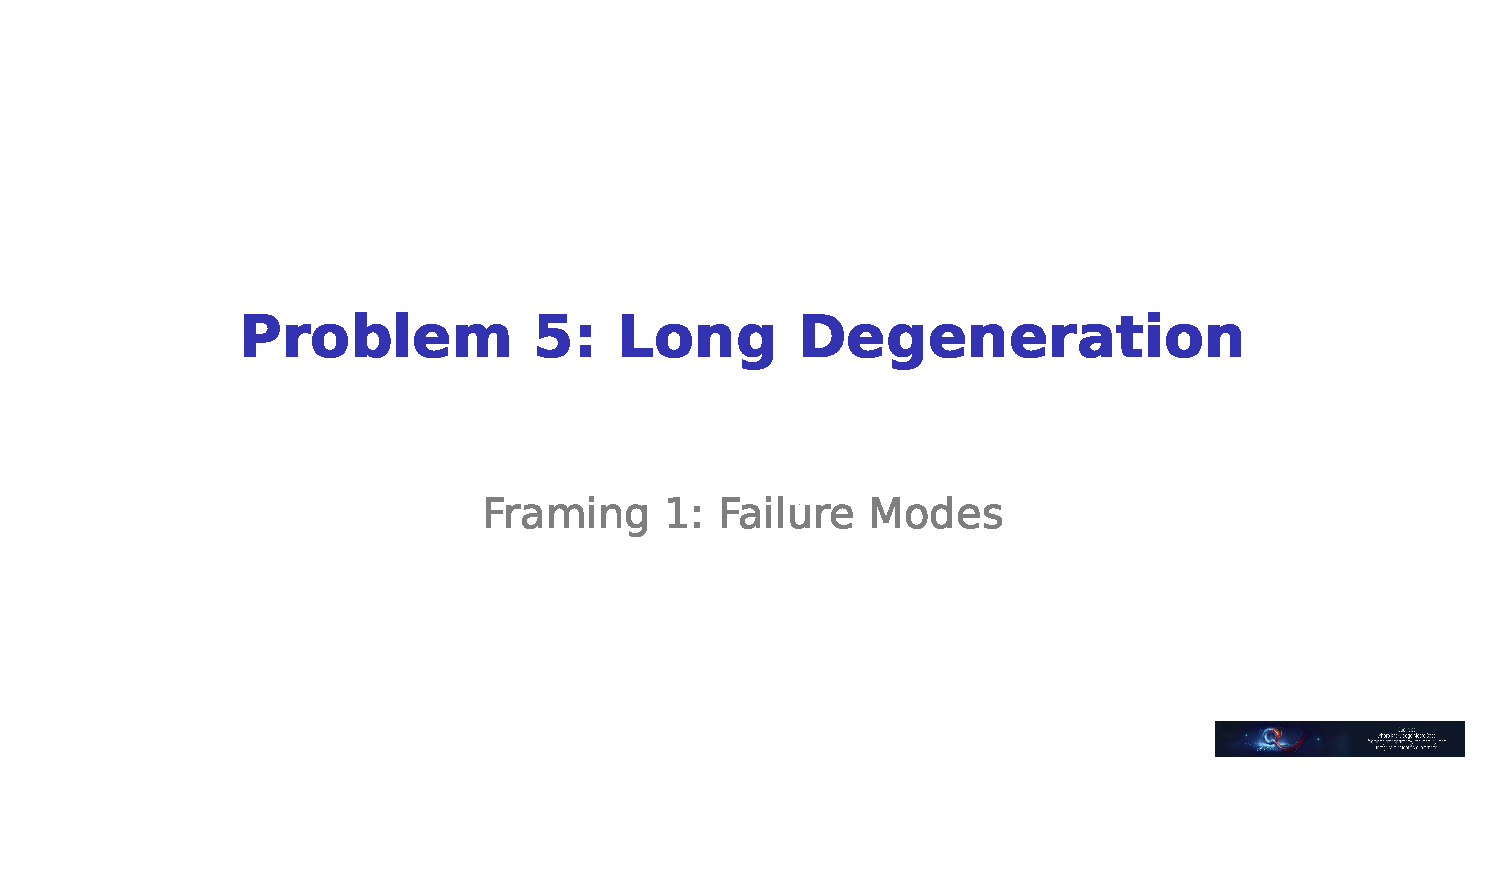
\includegraphics[width=0.95\textwidth]{../figures/framing1_problem5_long_degeneration.pdf}

Long texts repeat more

Models copy recent context

\column{0.48\textwidth}
\textbf{Solution}: \textcolor{mlpurple}{\textbf{CONTRASTIVE}}

Penalize similarity

$\alpha$ = 0.6 typical

Explicit degeneration prevention

\vspace{3mm}
\colorbox{green!20}{Best for long generation}
\end{columns}
\end{frame}

\begin{frame}{Framing 1, Problem 6: Quality-Diversity Tradeoff}
\begin{columns}
\column{0.48\textwidth}
\textbf{Problem}:


\includegraphics[width=0.95\textwidth]{../figures/framing1_problem6_quality_diversity.pdf}

Cannot maximize both

Fundamental tradeoff

\column{0.48\textwidth}
\textbf{Solution}: \textcolor{mlpurple}{\textbf{CHOOSE BY TASK}}

Translation → Beam

Creative → Nucleus/Contrastive

No universal best

\vspace{3mm}
\colorbox{green!20}{Task determines method}
\end{columns}
\end{frame}

% ============================================
% SECTION 2B: FRAMING 2 - TASK REQUIREMENTS
% ============================================

\begin{frame}{SECTION 2B: Framing 2 - Task Requirements}
\begin{center}
\Large
Frame as: ``What do we need and which method provides it''

\vspace{5mm}
6 needs → 6 methods

\vspace{5mm}
Next 6 slides show this framing
\end{center}
\end{frame}

\begin{frame}{Framing 2: 6 Needs (Summary)}
\small
\begin{enumerate}
\item Need exact/correct → GREEDY
\item Need better sequences → BEAM
\item Need creativity → TEMPERATURE
\item Need filter unlikely → TOP-K
\item Need adapt to distribution → NUCLEUS
\item Need prevent repetition → CONTRASTIVE
\end{enumerate}

\vspace{5mm}
\textbf{Pedagogical approach}: Positive framing (what we want to achieve)

vs Framing 1 (what goes wrong)
\end{frame}

% ============================================
% SECTION 2C: FRAMING 3 - PROGRESSIVE
% ============================================

\begin{frame}{SECTION 2C: Framing 3 - Progressive Sophistication}
\begin{center}
\Large
Frame as: ``Building up solutions progressively''

\vspace{5mm}
Start simple → Add sophistication → Solve harder problems

\vspace{5mm}
Shows natural evolution of methods
\end{center}
\end{frame}

\begin{frame}{Framing 3: Progressive Levels (Summary)}
\small
\begin{enumerate}
\item Level 1: Greedy too deterministic → Add Temperature
\item Level 2: Temperature too random → Add Top-k filtering
\item Level 3: Top-k inflexible → Dynamic Nucleus
\item Level 4: Still miss good paths → Beam exploration
\item Level 5: Still repetitive (long) → Contrastive penalty
\item Level 6: Need hybrid → Combine methods
\end{enumerate}

\vspace{5mm}
\textbf{Pedagogical approach}: Scaffolding (each method fixes previous limitation)
\end{frame}

% ============================================
% SECTION 2D: FRAMING 4 - BAD OUTPUTS
% ============================================

\begin{frame}{SECTION 2D: Framing 4 - Real Bad Outputs}
\begin{center}
\Large
Frame as: ``Here's actual bad output, here's the fix''

\vspace{5mm}
6 concrete failures → 6 targeted solutions

\vspace{5mm}
Most concrete/motivating approach
\end{center}
\end{frame}

\begin{frame}{Framing 4: Bad Outputs (Summary)}
\small
\begin{enumerate}
\item Output: ``city is a city in a city'' → FIX: Contrastive
\item Output: ``purple flying mathematics'' → FIX: Top-k/Nucleus
\item Output: Always same (boring) → FIX: Temperature
\item Output: Missed better sequence → FIX: Beam
\item Output: Wrong for distribution type → FIX: Nucleus
\item Output: Too slow for production → FIX: Greedy
\end{enumerate}

\vspace{5mm}
\textbf{Pedagogical approach}: Concrete examples first (most engaging)
\end{frame}

% ============================================
% RECOMMENDATIONS
% ============================================

\begin{frame}{RECOMMENDATIONS}
\textbf{My Recommendation}:

\vspace{5mm}
\textbf{Best Framing}: Framing 4 (Real Bad Outputs)

\textbf{Why}:
\begin{itemize}
\item Most concrete and motivating
\item Students see actual failures
\item Each method clearly solves specific problem
\item Memorable (students remember the bad examples)
\end{itemize}

\vspace{5mm}
\textbf{Best Setup Chart}: Option A (Bar Chart)

\textbf{Why}:
\begin{itemize}
\item Visual and quantitative
\item Shows distribution clearly
\item Easy to understand at a glance
\end{itemize}

\vspace{5mm}
\textbf{Structure}: 6 compact problem-solution slides + hybrid details (9 slides)

\textbf{Total Main}: ~20 slides (very focused and effective)
\end{frame}

\end{document}
